% \lipsum[2-3]

\section{Motivation}
\section{Aufgabenstellung}
\section{Zusammenfassung des Projektergebnisse}
\setauthor{Arsham Edalatkhah}
In den letzten Monaten haben wir an einer Reihe von Wettbewerben teilgenommen oder gewonnen, die unsere Kompetenz im Bereich der nachhaltigen Innovation und sozialen Unternehmerschaft unterstreichen. Hier sind die Details:

Linz-hACkT (11. bis 13. März 2023): 

Dies war ein Hackathon, der sich mit der Schaffung von Ideen und Visionen für eine klimaneutrale Stadt Linz bis 2040 beschäftigte. Wir haben an diesem Wettbewerb teilgenommen und konnten den ersten Platz erreichen. Dies hat uns die Chance gegeben, gute Verbindungen mit der Stadt Linz, dem Innovationshauptplatz Linz und Open Common Linz aufzubauen. Außerdem hatten wir die Chance, am 30. Jänner 2023 eine Präsentation für den Linzer Bürgermeister Klaus Luger und die Magistratsdirektorin Ulrike Huemer zu halten.

mPreneur Austria (22. September 2022): 

Im Rahmen des Projekts „mPreneur“ arbeiteten wir zusammen mit acht Organisationen weltweit, um ICT-Kompetenzen bei jungen Menschen aufzubauen. Wir haben an diesem Projekt teilgenommen und den ersten Platz gewonnen.

mPreneur Social Mobile Entrepreneurship (04. bis 09. November 2022): 

Dieses Projekt förderte die Kapazitätsentwicklung junger angehender Unternehmer und Jugend-CSOs. Ich, Arsham Edalatkhah, hatte die Chance, die Nochba App während des interkontinentalen Wettbewerbs "Social Mobile mPreneur" in Nord Mazedonien zu pitchen. Ich absolvierte im Vorfeld zwischen 6 und 8 Meetings mit Präsentationsexperten und konnte dadurch wertvolle Erfahrungen im Bereich der Präsentationstechnik sammeln.



\section{Projektvorgehensmodell}
\subsection{Projektorganisation}

\subsubsection{Discord}
\setauthor{Martin Hausleitner}
Die primäre Kommunikationsplattform zwischen dem Team und den Diplomarbeitbetreuer ist Discord. Da die Arbeit in den Sommerferien 2022 begonnen hat und zu diesem Zeitpunkt Corona-Regelungen galten, musste eine Meeting-Plattform gefunden werden, die sowohl Video- als auch Text-Chat ermöglicht. Aufgrund der Vertrautheit mit Discord und der Tatsache, dass es kostenlos ist, fiel die Entscheidung leicht.

Während der Diplomarbeit wurden über 40 Text-Kanäle erstellt, um alle relevanten Informationen, Notizen und Dokumentation zu speichern. Die Meeting-Notizen wurden jedoch auf ClickUp gespeichert.
\subsubsection{ClickUp}
\setauthor{Martin Hausleitner}
Um das Projekt effizient zu organisieren, wird nicht nur eine WhatsApp-Gruppe genutzt, sondern auch das Projektmanagement-Tool ClickUp. Die Entscheidung für ClickUp fiel leicht, da bereits viele Projektmanagement-Programme ausprobiert wurden und ClickUp bei den letzten Projekten am besten abgeschnitten hat. Außerdem ist es sehr intuitiv und einfach zu erlernen, was von beiden Team bestätigt wird.

\begin{figure}
    \centering
    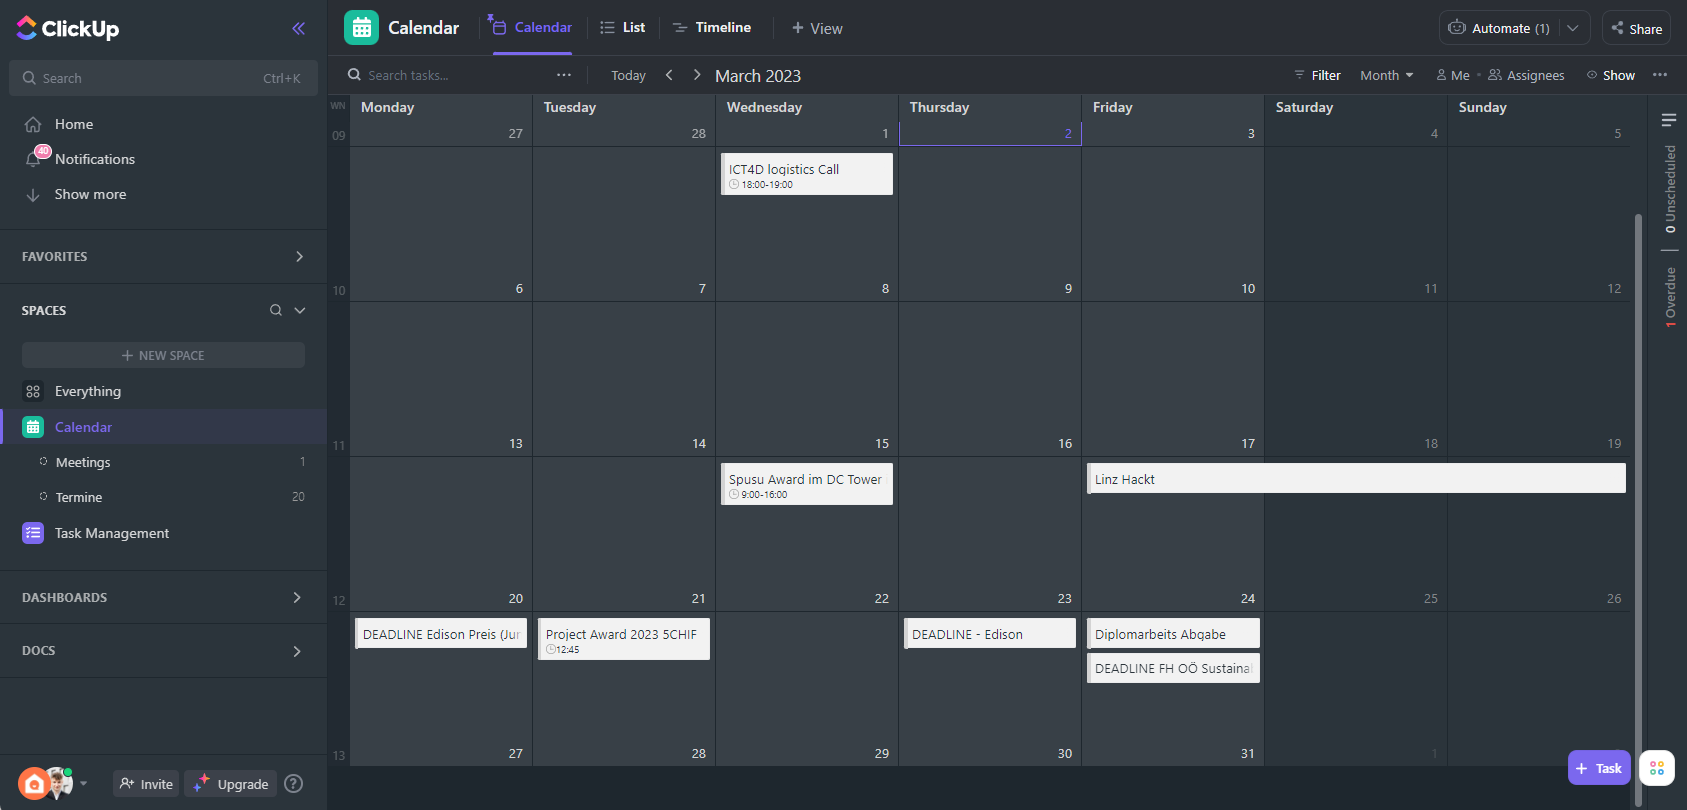
\includegraphics[width=1\textwidth]{./pics/clickup-calender-view.png}
    \caption{ClickUp Dashboard Kalender}
    \label{fig:clickup-calendar}
\end{figure}


In der Diplomarbeit wurden viele Mentoring-Sessions, Meetings mit dem Diplomarbeitbetreuer und weitere Termine wie Wettbewerbe vereinbart. Ohne eine geeignete Methode zur Verwaltung all dieser Termine kann es schnell unübersichtlich werden. Deshalb wurde das Kalender-Feature von ClickUp genutzt, um alle Einträge abzubilden, wie in Abbildung \ref{fig:clickup-calendar} zu sehen ist. Der Kalender wurde automatisch mit den persönlichen Kalendern synchronisiert, wie beispielsweise einem Google Kalender. Dadurch wurden nie Termine verpasst, was insbesondere dem Projektleiter sehr geholfen hat, da er nicht jeden daran erinnern musste, alle Termine in seinem Kalender einzutragen.

Ein weiterer wichtiger Punkt war das Task-Management in dem Projekt. Da im Projekt schnell viele Aufgaben koordiniert werden mussten, war es sinnvoll, alle Aufgaben in einer simplen To-Do-Liste abzubilden. Vor den Semesterferien wurde beispielsweise eine eigene Abteilung für Ferien-Tasks erstellt, um einen Überblick über alle Aufgaben während der Semesterferien zu haben. Obwohl die Tasks-To-Listen nicht aktiv genutzt wurden, war es sehr praktisch, um den Fortschritt zu überwachen und sicherzustellen, dass alles rechtzeitig erledigt wurde.

Zusammenfassend war ClickUp eine große Bereicherung für das
Projektmanagement, da es viel Zeit bei der Verwaltung von
Terminen und Aufgaben gespart hat. Auch die Benutzung als
neuer Benutzer war sehr einfach, sodass keine lange
Einarbeitungszeit nötig war. Besonders faszinierend ist,
dass ClickUp sehr intuitiv ist und viele nützliche Features
bietet.

